% --- LaTeX Lecture Notes Template - S. Venkatraman ---

% --- Set document class and font size ---

\documentclass[letterpaper, 12pt]{article}


% --- Package imports ---

% Extended set of colors
\usepackage[dvipsnames]{xcolor}

\usepackage{
  amsmath, amsthm, amssymb, mathtools, dsfont, units,          % Math typesetting
  graphicx, wrapfig, subfig, float,                            % Figures and graphics formatting
  listings, color, inconsolata, pythonhighlight,               % Code formatting
  fancyhdr, sectsty, hyperref, enumerate, enumitem, framed }   % Headers/footers, section fonts, links, lists

% lipsum is just for generating placeholder text and can be removed
\usepackage{hyperref, lipsum} 
% \usepackage{bm}
% \usepackage{subfig}

% --- Fonts ---

\usepackage{newpxtext, newpxmath, inconsolata}
\usepackage{amsfonts}
\usepackage{pgfplots}
\pgfplotsset{compat=1.12}
\usepackage{tkz-fct}
\usepackage{svg}
\usepackage{tikz}
\usepackage{tikz-cd}
\usepackage{lipsum}
\usepackage{enumitem}
\usepackage[title]{appendix}
% \usepackage[toc,page]{appxendix}
\usepackage[utf8]{inputenc}
\usepackage{multicol}
\usepackage{multirow}
\usepackage{booktabs}

\usepackage{minted}  % code highlighting
% \usepackage[finalizecache,cachedir=.]{minted}
% \usepackage[frozencache,cachedir=.]{minted}

\DeclareUnicodeCharacter{3BC}{$\pi$}
\DeclareUnicodeCharacter{3C0}{$\pi$}

\usepackage[most]{tcolorbox}
\newtcolorbox{myquote}[1][]{%
  colback=black!5,
  colframe=black!5,
  notitle,
  sharp corners,
  % borderline west={2pt}{0pt}{red!80!black},
  enhanced,
  breakable,
}

\renewcommand*\pod[1]{%
  \allowbreak
  \mathchoice
    {\mkern 18mu}%
    {\mkern  8mu}%
    {\mkern  6mu}% "6mu" matches the space *after* the word "mod"
    {\mkern  6mu}%
  (#1)%
}

% --- Page layout settings ---

% Set page margins
\usepackage[left=1.35in, right=1.35in, top=1.0in, bottom=.9in, headsep=.2in, footskip=0.35in]{geometry}

% Anchor footnotes to the bottom of the page
\usepackage[bottom]{footmisc}

% Set line spacing
\renewcommand{\baselinestretch}{1.2}

% Set spacing between paragraphs
\setlength{\parskip}{1.3mm}

% Allow multi-line equations to break onto the next page
\allowdisplaybreaks

% --- Page formatting settings ---

% Set image captions to be italicized
\usepackage[font={it,footnotesize}]{caption}

% Set link colors for labeled items (blue), citations (red), URLs (orange)
\hypersetup{colorlinks=true, linkcolor=RoyalBlue, citecolor=RedOrange, urlcolor=ForestGreen}

% Set font size for section titles (\large) and subtitles (\normalsize) 
\usepackage{titlesec}
% \titleformat{\section}{\large\bfseries}{{\fontsize{19}{19}\selectfont\textreferencemark}\;\; }{0em}{}
\titleformat{\section}{\large\bfseries}{\thesection\;\;\;}{0em}{}
\titleformat{\subsection}{\normalsize\bfseries\selectfont}{\thesubsection\;\;\;}{0em}{}

% Enumerated/bulleted lists: make numbers/bullets flush left
%\setlist[enumerate]{wide=2pt, leftmargin=16pt, labelwidth=0pt}
\setlist[itemize]{wide=0pt, leftmargin=16pt, labelwidth=10pt, align=left}

% --- Table of contents settings ---

\usepackage[subfigure]{tocloft}

% Reduce spacing between sections in table of contents
\setlength{\cftbeforesecskip}{.9ex}

% Remove indentation for sections
\cftsetindents{section}{0em}{0em}

% Set font size (\large) for table of contents title
\renewcommand{\cfttoctitlefont}{\large\bfseries}

% Remove numbers/bullets from section titles in table of contents
\makeatletter
\renewcommand{\cftsecpresnum}{\begin{lrbox}{\@tempboxa}}
\renewcommand{\cftsecaftersnum}{\end{lrbox}}
\makeatother

% --- Set path for images ---

\graphicspath{{Images/}{../Images/}}

% --- Math/Statistics commands ---

% Add a reference number to a single line of a multi-line equation
% Usage: "\numberthis\label{labelNameHere}" in an align or gather environment
\newcommand\numberthis{\addtocounter{equation}{1}\tag{\theequation}}

% Shortcut for bold text in math mode, e.g. $\b{X}$
\let\b\mathbf

% Shortcut for bold Greek letters, e.g. $\bg{\beta}$
\let\bg\boldsymbol

% Shortcut for calligraphic script, e.g. %\mc{M}$
\let\mc\mathcal

% \mathscr{(letter here)} is sometimes used to denote vector spaces
\usepackage[mathscr]{euscript}

% Convergence: right arrow with optional text on top
% E.g. $\converge[p]$ for converges in probability
\newcommand{\converge}[1][]{\xrightarrow{#1}}

% Weak convergence: harpoon symbol with optional text on top
% E.g. $\wconverge[n\to\infty]$
\newcommand{\wconverge}[1][]{\stackrel{#1}{\rightharpoonup}}

% Equality: equals sign with optional text on top
% E.g. $X \equals[d] Y$ for equality in distribution
\newcommand{\equals}[1][]{\stackrel{\smash{#1}}{=}}

% Normal distribution: arguments are the mean and variance
% E.g. $\normal{\mu}{\sigma}$
\newcommand{\normal}[2]{\mathcal{N}\left(#1,#2\right)}

% Uniform distribution: arguments are the left and right endpoints
% E.g. $\unif{0}{1}$
\newcommand{\unif}[2]{\text{Uniform}(#1,#2)}

% Independent and identically distributed random variables
% E.g. $ X_1,...,X_n \iid \normal{0}{1}$
\newcommand{\iid}{\stackrel{\smash{\text{iid}}}{\sim}}

% Sequences (this shortcut is mostly to reduce finger strain for small hands)
% E.g. to write $\{A_n\}_{n\geq 1}$, do $\bk{A_n}{n\geq 1}$
\newcommand{\bk}[2]{\{#1\}_{#2}}

\newcommand{\what}[1]{\widehat{#1}}
% \setcounter{section}{-1}

\setcounter{MaxMatrixCols}{20}

\newcommand{\SL}{\mathrm{SL}}
\newcommand{\Sp}{\mathrm{Sp}}
\newcommand{\Mp}{\mathrm{Mp}}
\newcommand{\GL}{\mathrm{GL}}
\newcommand{\SO}{\mathrm{SO}}
\newcommand{\SU}{\mathrm{SU}}
\newcommand{\PGL}{\mathrm{PGL}}
\newcommand{\PSL}{\mathrm{PSL}}
\newcommand{\GSp}{\mathrm{GSp}}
\newcommand{\PGSp}{\mathrm{PGSp}}
\newcommand{\Spin}{\mathrm{Spin}}
\newcommand{\gl}{\mathfrak{gl}}
\newcommand{\JL}{\mathrm{JL}}
\newcommand{\stab}{\mathrm{Stab}}
% \newcommand{\ab}{\mathrm{ab}}
\newcommand{\cha}{\mathrm{char}}
\newcommand{\fin}{\mathrm{fin}}
\newcommand{\Tr}{\mathrm{Tr}}
\newcommand{\Li}{\mathrm{Li}}
\newcommand{\trdeg}{\mathrm{trdeg}}
\newcommand{\rank}{\mathrm{rank}}
\newcommand{\rad}{\mathrm{rad}}
\newcommand{\Res}{\mathrm{Res}}
\newcommand{\Hom}{\mathrm{Hom}}
\newcommand{\Spec}{\mathrm{Spec}\,}
\newcommand{\Sym}{\mathrm{Sym}}
\newcommand{\ev}{\mathrm{ev}}
\newcommand{\disc}{\mathrm{disc}}
\newcommand{\Aut}{\mathrm{Aut}}
\newcommand{\Span}{\mathrm{Span}}
\newcommand{\supp}{\mathrm{supp}}
\newcommand{\sgn}{\mathrm{sgn}}
\newcommand{\Lie}{\mathrm{Lie}}
\newcommand{\Ind}{\mathrm{Ind}}
\newcommand{\pInd}{\mathrm{pInd}}
\newcommand{\Gal}{\mathrm{Gal}}
\newcommand{\Cl}{\mathrm{Cl}}
\newcommand{\Wh}{\mathrm{Wh}}
\newcommand{\std}{\mathrm{std}}
\newcommand{\Slit}{\mathrm{Slit}}
\newcommand{\pprod}{\sideset{}{'}\prod}
\newcommand{\potimes}{\sideset{}{'}\otimes}
\newcommand{\pbigotimes}{\sideset{}{'}\bigotimes}
% \sideset{}{'}\prod
\newcommand{\RQM}{\mathcal{RQM}}

\newcommand{\QM}{\mathcal{QM}}

\newcommand{\dd}{\mathrm{d}}
\newcommand{\dso}{\mathds{1}}

\newcommand{\llb}{\llbracket}
\newcommand{\rrb}{\rrbracket}

\newcommand{\rA}{\mathrm{A}}
\newcommand{\rB}{\mathrm{B}}
\newcommand{\rC}{\mathrm{C}}
\newcommand{\rD}{\mathrm{D}}
\newcommand{\rE}{\mathrm{E}}
\newcommand{\rF}{\mathrm{F}}
\newcommand{\rG}{\mathrm{G}}
\newcommand{\rH}{\mathrm{H}}
\newcommand{\rI}{\mathrm{I}}
\newcommand{\rJ}{\mathrm{J}}
\newcommand{\rK}{\mathrm{K}}
\newcommand{\rL}{\mathrm{L}}
\newcommand{\rM}{\mathrm{M}}
\newcommand{\rN}{\mathrm{N}}
\newcommand{\rO}{\mathrm{O}}
\newcommand{\rP}{\mathrm{P}}
\newcommand{\rQ}{\mathrm{Q}}
\newcommand{\rR}{\mathrm{R}}
\newcommand{\rS}{\mathrm{S}}
\newcommand{\rT}{\mathrm{T}}
\newcommand{\rU}{\mathrm{U}}
\newcommand{\rV}{\mathrm{V}}
\newcommand{\rW}{\mathrm{W}}
\newcommand{\rX}{\mathrm{X}}
\newcommand{\rY}{\mathrm{Y}}
\newcommand{\rZ}{\mathrm{Z}}

\newcommand{\bA}{\mathbb{A}}
\newcommand{\bB}{\mathbb{B}}
\newcommand{\bC}{\mathbb{C}}
\newcommand{\bD}{\mathbb{D}}
\newcommand{\bE}{\mathbb{E}}
\newcommand{\bF}{\mathbb{F}}
\newcommand{\bG}{\mathbb{G}}
\newcommand{\bH}{\mathbb{H}}
\newcommand{\bI}{\mathbb{I}}
\newcommand{\bJ}{\mathbb{J}}
\newcommand{\bK}{\mathbb{K}}
\newcommand{\bL}{\mathbb{L}}
\newcommand{\bM}{\mathbb{M}}
\newcommand{\bN}{\mathbb{N}}
\newcommand{\bO}{\mathbb{O}}
\newcommand{\bP}{\mathbb{P}}
\newcommand{\bQ}{\mathbb{Q}}
\newcommand{\bR}{\mathbb{R}}
\newcommand{\bS}{\mathbb{S}}
\newcommand{\bT}{\mathbb{T}}
\newcommand{\bU}{\mathbb{U}}
\newcommand{\bV}{\mathbb{V}}
\newcommand{\bW}{\mathbb{W}}
\newcommand{\bX}{\mathbb{X}}
\newcommand{\bY}{\mathbb{Y}}
\newcommand{\bZ}{\mathbb{Z}}

\newcommand{\bx}{\mathbf{x}}
\newcommand{\by}{\mathbf{y}}

\newcommand{\cA}{\mathcal{A}}
\newcommand{\cB}{\mathcal{B}}
\newcommand{\cC}{\mathcal{C}}
\newcommand{\cD}{\mathcal{D}}
\newcommand{\cE}{\mathcal{E}}
\newcommand{\cF}{\mathcal{F}}
\newcommand{\cG}{\mathcal{G}}
\newcommand{\cH}{\mathcal{H}}
\newcommand{\cI}{\mathcal{I}}
\newcommand{\cJ}{\mathcal{J}}
\newcommand{\cK}{\mathcal{K}}
\newcommand{\cL}{\mathcal{L}}
\newcommand{\cM}{\mathcal{M}}
\newcommand{\cN}{\mathcal{N}}
\newcommand{\cO}{\mathcal{O}}
\newcommand{\cP}{\mathcal{P}}
\newcommand{\cQ}{\mathcal{Q}}
\newcommand{\cR}{\mathcal{R}}
\newcommand{\cS}{\mathcal{S}}
\newcommand{\cT}{\mathcal{T}}
\newcommand{\cU}{\mathcal{U}}
\newcommand{\cV}{\mathcal{V}}
\newcommand{\cW}{\mathcal{W}}
\newcommand{\cX}{\mathcal{X}}
\newcommand{\cY}{\mathcal{Y}}
\newcommand{\cZ}{\mathcal{Z}}

\newcommand{\scA}{\mathscr{A}}
\newcommand{\scB}{\mathscr{B}}
\newcommand{\scC}{\mathscr{C}}
\newcommand{\scD}{\mathscr{D}}
\newcommand{\scE}{\mathscr{E}}
\newcommand{\scF}{\mathscr{F}}
\newcommand{\scG}{\mathscr{G}}
\newcommand{\scH}{\mathscr{H}}
\newcommand{\scI}{\mathscr{I}}
\newcommand{\scJ}{\mathscr{J}}
\newcommand{\scK}{\mathscr{K}}
\newcommand{\scL}{\mathscr{L}}
\newcommand{\scM}{\mathscr{M}}
\newcommand{\scN}{\mathscr{N}}
\newcommand{\scO}{\mathscr{O}}
\newcommand{\scP}{\mathscr{P}}
\newcommand{\scQ}{\mathscr{Q}}
\newcommand{\scR}{\mathscr{R}}
\newcommand{\scS}{\mathscr{S}}
\newcommand{\scT}{\mathscr{T}}
\newcommand{\scU}{\mathscr{U}}
\newcommand{\scV}{\mathscr{V}}
\newcommand{\scW}{\mathscr{W}}
\newcommand{\scX}{\mathscr{X}}
\newcommand{\scY}{\mathscr{Y}}
\newcommand{\scZ}{\mathscr{Z}}

\newcommand{\frA}{\mathfrak{A}}
\newcommand{\frB}{\mathfrak{B}}
\newcommand{\frC}{\mathfrak{C}}
\newcommand{\frD}{\mathfrak{D}}
\newcommand{\frE}{\mathfrak{E}}
\newcommand{\frF}{\mathfrak{F}}
\newcommand{\frG}{\mathfrak{G}}
\newcommand{\frH}{\mathfrak{H}}
\newcommand{\frI}{\mathfrak{I}}
\newcommand{\frJ}{\mathfrak{J}}
\newcommand{\frK}{\mathfrak{K}}
\newcommand{\frL}{\mathfrak{L}}
\newcommand{\frM}{\mathfrak{M}}
\newcommand{\frN}{\mathfrak{N}}
\newcommand{\frO}{\mathfrak{O}}
\newcommand{\frP}{\mathfrak{P}}
\newcommand{\frQ}{\mathfrak{Q}}
\newcommand{\frR}{\mathfrak{R}}
\newcommand{\frS}{\mathfrak{S}}
\newcommand{\frT}{\mathfrak{T}}
\newcommand{\frU}{\mathfrak{U}}
\newcommand{\frV}{\mathfrak{V}}
\newcommand{\frW}{\mathfrak{W}}
\newcommand{\frX}{\mathfrak{X}}
\newcommand{\frY}{\mathfrak{Y}}
\newcommand{\frZ}{\mathfrak{Z}}

\newcommand{\fra}{\mathfrak{a}}
\newcommand{\frb}{\mathfrak{b}}
\newcommand{\frc}{\mathfrak{c}}
\newcommand{\frd}{\mathfrak{d}}
\newcommand{\fre}{\mathfrak{e}}
\newcommand{\frf}{\mathfrak{f}}
\newcommand{\frg}{\mathfrak{g}}
\newcommand{\frh}{\mathfrak{h}}
\newcommand{\fri}{\mathfrak{i}}
\newcommand{\frj}{\mathfrak{j}}
\newcommand{\frk}{\mathfrak{k}}
\newcommand{\frl}{\mathfrak{l}}
\newcommand{\frm}{\mathfrak{m}}
\newcommand{\frn}{\mathfrak{n}}
\newcommand{\fro}{\mathfrak{o}}
\newcommand{\frp}{\mathfrak{p}}
\newcommand{\frq}{\mathfrak{q}}
\newcommand{\frr}{\mathfrak{r}}
\newcommand{\frs}{\mathfrak{s}}
\newcommand{\frt}{\mathfrak{t}}
\newcommand{\fru}{\mathfrak{u}}
\newcommand{\frv}{\mathfrak{v}}
\newcommand{\frw}{\mathfrak{w}}
\newcommand{\frx}{\mathfrak{x}}
\newcommand{\fry}{\mathfrak{y}}
\newcommand{\frz}{\mathfrak{z}}

\newcommand{\sage}{\raisebox{-0.16\height}{
\includegraphics[height=1em]{./sagelogo.png}}\,\,}

% Math mode symbols for common sets and spaces. Example usage: $\R$
\newcommand{\R}{\mathbb{R}}	% Real numbers
\newcommand{\C}{\mathbb{C}}	% Complex numbers
\newcommand{\Q}{\mathbb{Q}}	% Rational numbers
\newcommand{\Z}{\mathbb{Z}}	% Integers
\newcommand{\N}{\mathbb{N}}	% Natural numbers
\newcommand{\F}{\mathcal{F}}	% Calligraphic F for a sigma algebra
\newcommand{\El}{\mathcal{L}}	% Calligraphic L, e.g. for L^p spaces

% Math mode symbols for probability
\newcommand{\pr}{\mathbb{P}}	% Probability measure
\newcommand{\E}{\mathbb{E}}	% Expectation, e.g. $\E(X)$
\newcommand{\var}{\text{Var}}	% Variance, e.g. $\var(X)$
\newcommand{\cov}{\text{Cov}}	% Covariance, e.g. $\cov(X,Y)$
\newcommand{\corr}{\text{Corr}}	% Correlation, e.g. $\corr(X,Y)$
\newcommand{\B}{\mathcal{B}}	% Borel sigma-algebra

% Other miscellaneous symbols
\newcommand{\tth}{\text{th}}	% Non-italicized 'th', e.g. $n^\tth$
\newcommand{\Oh}{\mathcal{O}}	% Big-O notation, e.g. $\O(n)$
\newcommand{\1}{\mathds{1}}	% Indicator function, e.g. $\1_A$

\newcommand{\nul}{\mathrm{null}}
\newcommand{\range}{\mathrm{range}}

% Additional commands for math mode
\newcommand*{\argmax}{argmax}		% Argmax, e.g. $\argmax_{x\in[0,1]} f(x)$
\newcommand*{\argmin}{argmin}		% Argmin, e.g. $\argmin_{x\in[0,1]} f(x)$
\newcommand*{\spann}{Span}		% Span, e.g. $\spann\{X_1,...,X_n\}$
\newcommand*{\bias}{Bias}		% Bias, e.g. $\bias(\hat\theta)$
\newcommand*{\ran}{ran}			% Range of an operator, e.g. $\ran(T) 
\newcommand*{\dv}{d\!}			% Non-italicized 'with respect to', e.g. $\int f(x) \dv x$
\newcommand*{\diag}{diag}		% Diagonal of a matrix, e.g. $\diag(M)$
\newcommand*{\trace}{Tr}		% Trace of a matrix, e.g. $\trace(M)$
% \newcommand*{\supp}{supp}		% Support of a function, e.g., $\supp(f)$

% Numbered theorem, lemma, etc. settings - e.g., a definition, lemma, and theorem appearing in that 
% order in Lecture 2 will be numbered Definition 2.1, Lemma 2.2, Theorem 2.3. 
% Example usage: \begin{theorem}[Name of theorem] Theorem statement \end{theorem}
\theoremstyle{definition}
\newtheorem{theorem}{Theorem}[section]
\newtheorem{proposition}[theorem]{Proposition}
\newtheorem{lemma}[theorem]{Lemma}
\newtheorem{corollary}[theorem]{Corollary}
\newtheorem{definition}[theorem]{Definition}
\newtheorem{example}[theorem]{Example}
\newtheorem{question}[theorem]{Question}
\newtheorem{conjecture}[theorem]{Conjecture}
\newtheorem{exercise}[subsubsection]{Exercise}

\theoremstyle{remark}
\newtheorem{remark}[theorem]{Remark}

% Un-numbered theorem, lemma, etc. settings
% Example usage: \begin{lemma*}[Name of lemma] Lemma statement \end{lemma*}
\newtheorem*{theorem*}{Theorem}
\newtheorem*{proposition*}{Proposition}
\newtheorem*{lemma*}{Lemma}
\newtheorem*{corollary*}{Corollary}
\newtheorem*{definition*}{Definition}
\newtheorem*{example*}{Example}
\newtheorem*{remark*}{Remark}
\newtheorem*{claim}{Claim}
\newtheorem*{conjecture*}{Conjecture}

% --- Left/right header text (to appear on every page) ---

% Do not include a line under header or above footer
\pagestyle{fancy}
\renewcommand{\footrulewidth}{0pt}
\renewcommand{\headrulewidth}{0pt}

% Right header text: Lecture number and title
\renewcommand{\sectionmark}[1]{\markright{#1} }
% \fancyhead[R]{\small\textit{\nouppercase{\rightmark}}}

% Left header text: Short course title, hyperlinked to table of contents
% \fancyhead[L]{\hyperref[sec:contents]{\small Matrix multplication}}

% \pgfkeys{/Dynkin diagram,
% edge length=1.5cm,
% fold radius=1cm,
% indefinite edge/.style={
% draw=black,
% fill=white,
% thin,
% densely dashed}}

\usepackage{fancyhdr}
\pagestyle{fancy}
\fancyhead[R]{}
\fancyhead[L]{}


% start section number from 0
\setcounter{section}{-1}

% --- Document starts here ---

\begin{document}

% --- Main title and subtitle ---

\title{Irrationality proofs using modular forms \\[1em]
\normalsize Re-\TeX ed by Seewoo Lee\footnote{seewoo5@berkeley.edu. Some typos are fixed with footnotes.}}
% \\[1em]
% \normalsize Re-typed by Seewoo Lee\footnote{seewoo5@berkeley.edu}}

% --- Author and date of last update ---

\author{Frits Beukers}
\date{\normalsize\vspace{-1ex} Last updated: \today}

% --- Add title and table of contents ---

\maketitle


% --- Abstracts ---

% \tableofcontents\label{sec:contents}

\section{Introduction}

In the years following Apery's discovery of his irrationality proofs for $\zeta(2), \zeta(3)$ (see \cite{van1979proof}), it has become clear that these proofs do not only have significance as irrationality proofs, but the numbers that occur in them serve as interesting examples for several phenomena in algebraic geometry and modular form theory.
See \cite{gessel1982some,beukers1982irrationality,beukers1985some,beukers1987another} for congruences of the Ap\'ery numbers and \cite{beukers1984family,stienstra1985picard} for geometrical and modular interpretations.\footnote{The original citations were in a different order, but it seems that this is the correct order.}
Furthermore, it turns out that Apery's proofs themselves are in fact simple consequences of elementary complex analysis on spaces of certain modular forms.
In the present paper we describe this analysis together with some generalisations in Theorems 1 to 5. 
For example, we prove that $8\zeta(3) - 5 \sqrt{5} L(3) \not \in \bQ(\sqrt{5})$, where $L(3) = \sum_{n=1}^{\infty} \left(\frac{n}{5}\right) n^{-3}$.
Although the use of modular forms in irrationality proofs looks promising at first sight, the yield of new irrationality results thus far is disappointingly low. 
However, in methods such as this it is easy to overlook some simple tricks that may give new interesting results.

The first section of this paper describes the general framework of the proofs.
This section may seem vague at first sight, but in combination with the proof of Theorem 1 we hope that things will be clear.
We have given the proof of Theorem 1 as extensively as possible in order to set it as an example for the other proofs, where we omit some minor details now and then. 
\section{Preliminaries}

In this section we shall describe the general principles which are used in the arguments of the following sections.

Let $t(q) = \sum_{n=0}^{\infty} t_n q^n$ a power series convergent for all $|q| < 1$.
Let $w(q)$ be another analytic function on $|q| < 1$.
We like to study $w$ as function of $t$.
In general it will be a multivalued function over which we have no control.
However, we shall introduce some assumptions.
First, $t_0 = 0, t_1 \ne 0$.
Let now $q(t)$ be the local inverse of $t(q)$ with $q(0) = 0$.
Choose $w(q(t))$ for the value of $w$ around $t = 0$.
In order to determine the radius of convergence of the powerseries $w(q(t)) = \sum_{n=0}^{\infty} w_n t^n$ we introduce branching values of $t$.
We say that $t$ branches above $t_0$, if either $t_0$ is not in the image of $t$, or if $t'(q_0) = 0$ for some $q_0$ with $t(q_0) = t_0$.
In other words, $t$ branches above $t_0$, if the map $t : \{|q| < 1\} \to \bC$ is not a local covering above $t_0$.
We call such a $t_0$ a branching value of $t$.
Now assume, that $t$ has a discrete set of branching values $t_1, t_2, \dots$ where we have excluded zero as a possible value and suppose $|t_1| < |t_2| < \dots$.
It is clear now that the radius of convergence is in general $|t_1|$.
We shall be interested in cases where the radius of convergence is larger than $|t_1|$.
Let $\gamma$ be a closed contour in the complex $t$-plane beginning and ending at the origin, not passing through any $t_i$ and which encircles the point $t_1$ exactly once.
Suppose that analytic continuation of $w(q(t))$ along $\gamma$ again yields the same branch of $w(q(t))$.
Then $w(q(t))$ can be continued analytically to the disc $|t| < |t_2|$ with exception of the possible isolated singularity $t_1$.
If $w(q(t))$ remains bounded around we can conclude that the radius of convergence is at least $t_2$.
Our irrationality proofs consist exactly of the construction of such instances.
The point of having a radius of convergence as large as possible consists of the following Proposition.

\begin{proposition}
    \label{prop:1.1}
    Let $f_0(t), f_1(t), \dots, f_k(t)$ be power series in $t$.
    Suppose that for any $n \in \bN$, $i = 0, 1, \dots, k$ the $n$-th coefficient in the Taylor series of is rational and has denominator dividing $d^n [1, \dots, n]^r$
     where $r, d$ are certain fixed positive integers and $[1, \dots, n]$ is the lowest common multiple of $1, \dots, n$.
    Suppose there exist real numbers $\theta_1, \dots, \theta_k$ such that $f_0(t) + \theta_1 f_1(t) + \cdots + \theta_k f_k(t)$ has radius of convergence $\rho$ and infinitely many nonzero Taylor coefficients.
    If $\rho > d e^r$, then at least one of $\theta_1, \dots, \theta_k$ is irrational.
\end{proposition}

\begin{remark*}
    Note that if $k = 1$ we have an honest irrationality proof.
\end{remark*}

\begin{proof}
    Choose $\epsilon > 0$ such that $\rho - \epsilon > d e^{r(1 + \epsilon)}$.
    Let $f_i = \sum_{n=0}^{\infty} a_{i,n} t^n$.
    Since the radius of the convergence of $f_0 + \theta_1 f_1 + \cdots + \theta_k f_k$ is $\rho$,
    we have for sufficiently large $n$, $|a_{0,n} + \theta_1 a_{1,n} + \cdots + \theta_k a_{k,n}| \le (\rho - \epsilon)^{-n}$.
    Suppose $\theta_1, \dots, \theta_k$ are all rational and have common denominator $D$.
    Then $A_n = D d^n [1, \dots, n]^r |a_{0,n} + \theta_1 a_{1,n} + \cdots + \theta_k a_{k,n}|$ is an integer smaller than
    $D d^n [1, \dots, n]^r (\rho - \epsilon)^{-n}$.
    By the prime number theorem we have $[1, \dots, n] < e^{(1 + \epsilon)n}$ for sufficiently large $n$,
    hence $A_n < D (d e^{r(1 + \epsilon)} (\rho - \epsilon)^{-1})^{n}$.
    Since $d e^{r(1 + \epsilon)}  (\rho - \epsilon)^{-1} < 1$ this implies that $A_n = 0$ for sufficiently large $n$,
    in contradiction with the assumption $A_n \ne 0$ for infinitely many $n$.
    Thus our proposition follows. 
\end{proof}

The construction of the functions $t(q)$ and $w(q)$ will proceed using
modular forms and functions. The values for which we obtain irrationality
results are in fact values at integral points of Dirichlet series
associated to modular forms.

\begin{proposition}
    \label{prop:1.2}
    Let $F(\tau) = \sum_{n=1}^{\infty} a_n q^n$, $q = e^{2 \pi i \tau}$ be a Fourier series
    convergent for $|q| < 1$, such that for some $k, n \in \bN$,
    $$
        F\left(-\frac{1}{N\tau}\right) = \varepsilon(-i\tau \sqrt{N})^{k} F(\tau)
    $$
    where $\varepsilon = \pm 1$.
    Let $f(\tau)$ be the Fourier series
    $$
        f(\tau) = \sum_{n = 1}^{\infty} \frac{a_n}{n^{k-1}} q^n.
    $$
    Let
    $$
        L(F, s) = \sum_{n=1}^{\infty} \frac{a_n}{n^s}
    $$
    and finally,
    $$
        h(\tau) = f(\tau) - \sum_{0 \le r < \frac{1}{2}(k - 2)} \frac{L(F, k - r - 1)}{k!} (2 \pi i \tau)^r.
    $$
    Then
    $$
        h(\tau) - D = (-1)^{k-1} \varepsilon (-i\tau \sqrt{N})^{k-2} h\left(-\frac{1}{N\tau}\right)
    $$
    where $D = 0$ if $k$ is odd and $D = L(F, \frac{1}{2}k) (2 \pi i \tau)^{\frac{1}{2}k - 1} / (\frac{1}{2}k - 1)!$ if $k$ is even.
    Moreover, $L(F, \frac{1}{2}k) = 0$ if $\varepsilon = -1$.
\end{proposition}

\begin{proof}
    We apply a lemma of Hecke, see \cite[Section 5]{weil1977remarks} with $G(\tau) = \varepsilon F(\tau) / (i \sqrt{N})^k$ to obtain
    $$
        f(\tau) - \varepsilon(-1)^{k-1} (-i \tau \sqrt{N})^{k-2} f\left(-\frac{1}{N\tau}\right) = \sum_{r = 0}^{k-2} \frac{L(F, k - r - 1)}{r!} (2 \pi i \tau)^r.
    $$
    Split the summation on the right hand side into summations over $r < \frac{1}{2}k - 1$, $r > \frac{1}{2}k - 1$ and,
    possibly, $r = \frac{1}{2}k - 1$.
    For the region $r > \frac{1}{2}k - 1$ we apply the functional equation
    $$
        \frac{L(F, k - r - 1)}{r!} = \varepsilon (-1)^{k} (-i\sqrt{N})^{k-2} \left(-\frac{1}{N}\right)^{k-r-2} (2 \pi i )^{k- 2r - 2} \frac{L(F, r + 1)}{(k - r - 2)!}
    $$
    and substitute $r$ by $k - 2 - r$.
\end{proof}

\section{The group $\Gamma_1(6)$}

This group is exactly the subgroup of $\SL_2(\bZ)$ of all matrices $(\begin{smallmatrix}
    a & b \\ c & d
\end{smallmatrix})$ with $a \equiv d \equiv 1 \pmod{6}$, $c \equiv 0 \pmod{6}$.
Its fundamental domain can be pictured as below.

% Inspired from https://tex.stackexchange.com/a/661303/111403
\begin{center}
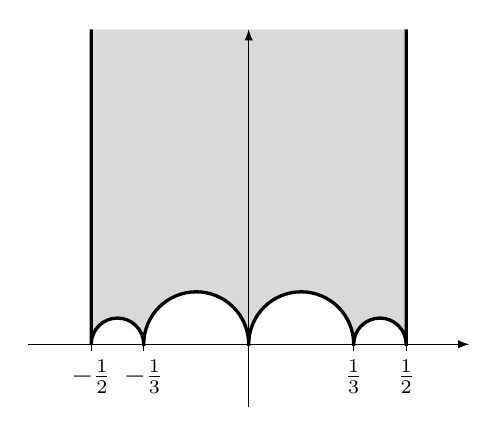
\begin{tikzpicture}[scale=4]
    \draw[very thick, fill=gray!30]
        (-.5,1) -- (-.5,0) --
        (-1/2, 0) arc (180:0:1/12) --
        (-1/3, 0) arc (180:0:1/6) --
        (0, 0) arc (180:0:1/6) --
        (1/3, 0) arc (180:0:1/12) --
        (.5, 0) -- (.5,1);
    \draw[-latex] (-0.7,0) -- (0.7,0);
    \draw[-latex] (0,-.2) -- (0,1);
    \draw(-.5,.02)--(-.5,-.02)node[below]{$-\frac{1}{2}$};
    \draw(.5,.02)--(.5,-.02)node[below]{$\frac{1}{2}$};
    \draw(-1/3,.02)--(-1/3,-.02)node[below]{$-\frac{1}{3}$};
    \draw(1/3,.02)--(1/3,-.02)node[below]{$\frac{1}{3}$};
\end{tikzpicture}
\end{center}
A complete set of inequivalent cusps is given by $0, 1/2, 1/3, \infty$.
They are regular and have widths 6, 3, 2, 1 respectively.
Consider the following function,
$$
    y(\tau) = \frac{\eta(6\tau)^8 \eta(\tau)^4}{\eta(2\tau)^6 \eta(3\tau)^4}
$$
where
$$
    \eta(\tau) = q^{1/24} \prod_{n=1}^{\infty} (1 - q^n), \quad q = e^{2\pi i \tau}, \quad \tau \in \bH.
$$
That it is a modular function on $\Gamma_1(6)$ can be checked using the tranformation formula for $\eta(\tau)$ in \cite[Ch 9]{rademacher2012topics}.
Since $y(\tau)$ has only one simple zero in the fundamental domain it generates the field of modular functions on $\Gamma_1(6)$.
Moreover, $y(0) = 1/9$, $y(1/3) = 1$, $y(1/2) = \infty$, $y(\infty) = 0$.
The function $y(-1/6\tau)$ is again invariant on $\Gamma_1(6)$ and one easily checks that
\begin{equation}
    \label{eqn:1}
    y\left(-\frac{1}{6\tau}\right) = \frac{y(\tau) - 1/9}{y(\tau) - 1}.
\end{equation}
Hence the function
$$
    t(\tau) = y(\tau) \frac{1 - 9y(\tau)}{1 - y(\tau)}
$$
is invariant under the involution $\tau \mapsto -1/6\tau$.
Moreover,
$$
    t(\tau) = \left(\frac{\Delta(6\tau) \Delta(\tau)}{\Delta(3\tau) \Delta(2\tau)}\right)^{1/2} = q \prod_{n = 0}^{\infty} (1 - q^{6n + 1})^{12} (1 - q^{6n + 5})^{-12}
$$
which is checked by noticing that $(\Delta(6\tau) \Delta(\tau) / \Delta(3\tau) \Delta(2\tau))^{1/2}$ is modular with respect to $\Gamma_1(6)$, invariant under $\tau \mapsto -1/6\tau$ and its zeros and poles coincide with those of $t(\tau)$.

\begin{proposition}
\label{prop:2.1}
    The function $t(\tau)$ maps the shaded open area in the picture below univalently onto the upper half plane and satisfies
    $$
        t(i\infty) = 0, \quad t\left(\frac{i}{\sqrt{6}}\right) = (\sqrt{2} - 1)^{4}, \quad t\left(\frac{2}{5} + \frac{i}{5\sqrt{6}}\right) = (\sqrt{2} + 1)^{4},\quad t\left(\frac{1}{2}\right) = \infty.
    $$
\end{proposition}
\begin{center}
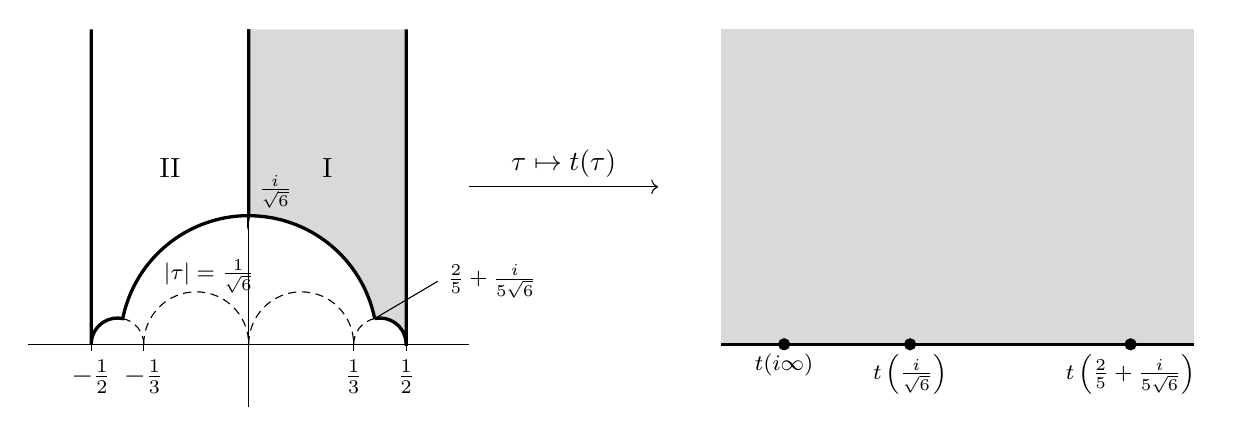
\begin{tikzpicture}[scale=4]
    \draw[very thick]
        (-.5,1) -- (-.5,0) --
        (-1/2, 0) arc (180:78.5:1/12) --
        (-2/5, {1/(5 * sqrt(6))}) arc (168.5:90:{1/sqrt(6)}) --
        (0,{1/sqrt(6)}) -- (0,1);
    \draw[very thick, fill=gray!30]
        (0,1) --
        (0, {1/sqrt(6)}) arc (90:11.5:{1/sqrt(6)}) --
        (2/5, {1/(5 * sqrt(6))}) arc (101.5:0:1/12) --
        (1/2,0) -- (1/2,1);
    \draw (-0.7,0) -- (0.7,0);
    \draw (0,-.2) -- (0,1);
    \draw (0,0.4)node[above right, font=\footnotesize]{$\frac{i}{\sqrt{6}}$};
    \draw[densely dashed] (-1/3, 0) arc (0:78.5:1/12);
    \draw[densely dashed] (-1/3,0) arc (180:0:1/6);
    \draw[densely dashed] (1/3,0) arc (180:101.5:1/12);
    \draw[densely dashed] (0,0) arc (180:0:1/6);
    \draw(-.5,.02)--(-.5,-.02)node[below]{$-\frac{1}{2}$};
    \draw(.5,.02)--(.5,-.02)node[below]{$\frac{1}{2}$};
    \draw(-1/3,.02)--(-1/3,-.02)node[below]{$-\frac{1}{3}$};
    \draw(1/3,.02)--(1/3,-.02)node[below]{$\frac{1}{3}$};
    \draw (2/5, {1/(5 * sqrt(6))}) -- (0.6,0.2)node[right, font=\footnotesize]{$\frac{2}{5} + \frac{i}{5\sqrt{6}}$};
    \draw (-0.25, 0.5)node[above]{II};
    \draw (0.25, 0.5)node[above]{I};
    \draw (-0.3, 0.3)node[below right, font=\footnotesize]{$|\tau| = \frac{1}{\sqrt{6}}$};

    \draw[->] (0.7,0.5) -- (1.3,0.5);
    \draw (1.0, 0.5)node[above]{$\tau \mapsto t(\tau)$};

    \fill[gray!30] (1.5,1.0) -- (1.5,0) -- (3.0, 0) -- (3.0, 1.0);
    \draw[very thick] (1.5,0) -- (3,0);
    \draw[fill] (1.7,0) circle (0.5pt)node[below, font=\footnotesize]{$t(i\infty)$};
    \draw[fill] (2.1,0) circle (0.5pt)node[below, font=\footnotesize]{$t\left(\frac{i}{\sqrt{6}}\right)$};
    \draw[fill] (2.8,0) circle (0.5pt)node[below, font=\footnotesize]{$t\left(\frac{2}{5}+\frac{i}{5\sqrt{6}}\right)$};
\end{tikzpicture}
\end{center}

\begin{proof}
That $t(i \infty) = 0$, $t(\frac{1}{2}) = \infty$ can be ssen from the values $y(i\infty) = 0$, $y(\frac{1}{2}) = \infty$.
From \eqref{eqn:1} it follows that for $\tau = i/\sqrt{6}$ and $y_0 = y(\frac{i}{\sqrt{6}})$, we have $y_0 = \frac{y_0 - \frac{1}{9}}{y_0 - 1}$, hence $y_0 = 1 \pm \frac{2 \sqrt{2}}{3}$ and correspondingly, $t(\frac{i}{\sqrt{6}}) = (\sqrt{2} \pm 1)^4$.
The same principle can be applied to obatin $t(\frac{2}{5} + \frac{i}{5\sqrt{6}}) = (\sqrt{2} \pm 1)^4$.
To decide which sign should be taken, one estimates $t(\frac{i}{\sqrt{6}})$ and $t(\frac{2}{5} + \frac{i}{5\sqrt{6}})$ numerically and obtain the values of our proposition.
Furthermore, $t(\tau)$ assumes every value at most once in the union of I and II.
Our proposition now follows.
\end{proof}

In the theorems and proofs that follow we let $\rM_k(\Gamma_1(6))$ be the space of modular forms of weight $k$ with respect to $\Gamma_1(6)$, and let
$$
    E_4 (\tau) = 1 + 240 \sum_{n=1}^{\infty} \sigma_3(n) q^n, \quad E_2(\tau) = 1 - 24 \sum_{n=1}^{\infty} \sigma_1(n) q^n 
$$
be the standard Eisenstein series.

\begin{theorem}
    \label{thm:1}
    $\zeta(3)$ is irrational.
\end{theorem}

\begin{proof}
    Let
    \begin{align*}
        40 F(\tau) &= E_4(\tau) - 36 E_4(\tau) - 7 (4E_4(2\tau) - 9E_4(3\tau)) \\
        24 E(\tau) &= -5(E_2(\tau) - 6E_2(6\tau)) + 2E_2(2\tau) - 3E_2(3\tau).
    \end{align*}
    Notice that $F(\tau) \in \rM_4(\Gamma_1(6))$ and $F(-1/6\tau) = -36 \tau^4 F(\tau)$, $F(i\infty) = 0$ and $E(\tau) \in \rM_2(\Gamma_1(6))$, $E(-1/6\tau) =  - 6\tau^2 E(\tau)$.
    The Dirichlet series corresponding to $F(\tau)$ reads
    \begin{align*}
        L(F, s) &= \sum_{n=1}^{\infty} \frac{6\sigma_3(n)}{n^s} - 36 \frac{6 \sigma_3(n)}{(6n)^s} - 28 \frac{6 \sigma_3(n)}{(2n)^s} + 63 \frac{6 \sigma_3(n)}{(3n)^s} \\
        &= 6(1 - 6^{2-s} - 7 \cdot 2^{2-s} + 7 \cdot 3^{2-s}) \zeta(s) \zeta(s - 3).
    \end{align*}
    Define $f(\tau)$ by $(\frac{\dd}{\dd \tau})^{3} f(\tau) = (2 \pi i )^{3} F(\tau)$, $f(i \infty) = 0$.
    From Proposition \ref{prop:1.2} and the fact that $F(-1/6\tau) = -36 \tau^4 F(\tau)$ follows\footnote{There's a typo in the original article: $L(F, s)$ should be $L(F, 3)$.}
    $$
        6 \tau^2 \left(f\left(-\frac{1}{6\tau}\right) - L(F, 3)\right) = -(f(\tau) - L(F, 3))
    $$
    and since $L(F, 3) = 6 \cdot (-1/3) \zeta(3) \zeta(0) = \zeta(3)$, we have
    $$
        6 \tau^2 \left(f\left(-\frac{1}{6\tau}\right) - \zeta(3)\right) = -(f(\tau) - \zeta(3)).
    $$
    Multiplication with $E(-1/6\tau) = -6\tau^2 E(\tau)$ gives
    \begin{equation}
        \label{eqn:2}
        E\left(-\frac{1}{6\tau}\right) \left(f\left(-\frac{1}{6 \tau}\right) - \zeta(3)\right) = E(\tau) (f(\tau) - \zeta(3)).
    \end{equation}
    The function $E(\tau)(f(\tau) - \zeta(3))$ can be considered as a multivalued function of $t = t(\tau)$.
    We choose it at $t = 0$ as follows.
    From the expansion $t = q\prod_{n=1}^{\infty} (1 - q^{6n + 1})^{12} (1 - q^{6n + 5})^{-12} = q - 12q^2 = 66q^3 - 220q^4 + 495 q^5 - \dots$ one infres the inverse expansion $q = t + 12 t^2 + 222 t^3 + \dots$.
    Then, from $E(\tau) = 1 + 5q + 13 q^2 + \dots$ one finds $E(t) = 1 + 5t + 73 t^2 + 1445 t^3 + \dots$ and similarly, $E(t) F(t) = 6t + (351/4)t^2 + \dots$.

    By construction one notes that $E(t) \in \bZ\llbracket t\rrbracket$ and  and $E(t) f(t) = \sum_{n=1}^{\infty} a_n t^n$ where $a_n \in \bZ / [1, \dots, n]^3$.
    Since the inverse function $t \to \tau$ branches at $(\sqrt{2} - 1)^{4}$ one expects the radius of convergence of $E(t)(f(t) - \zeta(3))$ to be $(\sqrt{2} - 1)^{4}$.
    However, by the property \eqref{eqn:2}, the function $t \mapsto E(t) (f(t) - \zeta(3))$ has no branch point at $t = (\sqrt{2} - 1)^4$, and its radius of convergence equals at least the next branching value, which is $(\sqrt{2} + 1)^{4}$.
    Furthermore, it cannot be a polynomial in $t$, since then $f(\tau) - \zeta(3)$ would be a modular form of weight $-2$, which is impossible.
    We now apply Proposition \ref{prop:1.1} with $\theta_1 = \zeta(3)$ to conclude $\zeta(3) \not \in \bQ$.
\end{proof}

\begin{remark*}
    Note that $1, 5, 73, 1445, \dots$ are exactly Ap\'ery's numbers for $\zeta(3)$.
\end{remark*}

\begin{theorem}
    \label{thm:2}
    Let $F(\tau)  = \eta(\tau)^{2} \eta(2\tau)^{2} \eta(3\tau)^{2} \eta(6\tau)^2$ and $L(F, s)$ the corresponding Dirichlet series.
    Then at least one of the numbers $\pi^{-2}L(F, 2)$ and $L(F, 3) + 47 L(F, 2) \zeta(3) / 48 \pi^2$ is irrational.
\end{theorem}

\begin{proof}
    The function $F(\tau)$ is in $\rM_4(\Gamma_1(6))$, it is a cusp form, and $F(-1/6\tau) = 36 \tau^4 F(\tau)$.
    Let $f(\tau)$ be the Fourier series such that $(\frac{\dd}{\dd \tau})^{3} f(\tau) = (2 \pi i )^{3} F(\tau)$, $f(i \infty) = 0$.
    Then it follows from Proposition \ref{prop:1.2} that
    \begin{equation}
        \label{eqn:3}
        6 \tau^2 \left(f\left(-\frac{1}{6\tau}\right) - L(F, 3)\right) = f(\tau) - L(F, 3) - L(F, 2) (2 \pi i \tau).
    \end{equation}
    Consider also
    $$
        240 G(\tau) = 13 (E_4(\tau) + 36 E_4(6\tau)) - 37 (4E_4(2\tau) + 9E_4(3\tau)).
    $$
    It ahs the properties $G(i\infty) = 0$, $G(-1/6\tau) = 36 \tau^4 G(\tau)$.
    The corresponding Dirichlet series reads
    $$
        L(G, s) = (13 + 13 \cdot 6^{2-s} - 37 \cdot 2^{2-s} - 37 \cdot 3^{2-s}) \zeta(s) \zeta(s - 3).
    $$
    Letting $(\frac{\dd}{\dd \tau})^{3} g(\tau) = (2\pi i)^{3} G(\tau)$, $g(i\infty) = 0$, we have
    $$
        6 \tau^2 \left(g\left(-\frac{1}{6\tau}\right) - L(G, 3)\right) = g(\tau) - L(G, 3) - L(G, 2) (2 \pi i \tau),
    $$
    hence,
    \begin{equation}
        \label{eqn:4}
        6 \tau^2 \left(g\left(-\frac{1}{6\tau}\right) - \frac{47}{3}\zeta(3)\right) = g(\tau) - \frac{47}{6} \zeta(3) + 48 \zeta(2) (2\pi i \tau).
    \end{equation}
    Elimination of $2\pi i \tau$ form \eqref{eqn:3} and \eqref{eqn:4} gives that the function $h(\tau) = 48 \zeta(2) (f(\tau) - L(F, 3)) + L(F, 2) (g(\tau) - \frac{47}{6}\zeta(3))$ behaves like $6 \tau^2 h(-1/6 \tau) = h(\tau)$.
    Now consider
    $$
        E(\tau) = E_2(\tau) - 2E_2(2 \tau) + 6 E_2(3\tau) - 3 E_2(6\tau).
    $$
    It is in $\rM_2(\Gamma_1(6))$ and we have $E(-1/6\tau) = 6 \tau^2 E(\tau)$.
    Consequently, $E(-1/6\tau) h(-1/6\tau) = E(\tau) h(\tau)$ and by an argument to the one in Theorem \ref{thm:1} we find that
    $$
        48 \zeta(2) f(t) E(t) + L(F, 2) g(t) E(t) - \left(48 \zeta(2) L(F, 3) + L(F, 2) \frac{47}{6} \zeta(3) \right) E(t)
    $$
    is a power series in $t$ with radius of convergence $(\sqrt{2} + 1)^4$.
    Again the denominator of the $n$-th coefficient in the power series of $E(t) f(t)$, $E(t) g(t)$, $E(t)$ divides $[1, \dots, n]^3$.
    We can now apply Proposition \ref{prop:1.1} to obtain our theorem.
\end{proof}

\begin{theorem}
    \label{thm:3}
    Let
    $$
        \sum_{n=1}^{\infty} a_n q^n = \left(\frac{\eta^9(\tau) \eta^9 (6\tau)}{\eta^3(2\tau) \eta^3(3 \tau)}\right)^{\frac{1}{2}} = q \prod_{n=1}^{\infty} (1 - q^n)^{3} (1 - q^{3n})^{3} \frac{(1 + q^{3n})^{\frac{9}{2}}}{(1 + q^{n})^{\frac{3}{2}}}.
    $$
    Then $\sum_{n=1}^{\infty} a_n / n^{2}$ is irrational.
\end{theorem}

\begin{proof}
    Consider the product
    $$
        E(\tau) = \frac{\eta^7(2\tau) \eta^7(3 \tau)}{\eta^5(\tau) \eta^5(6\tau)}.
    $$
    We have $E(-1/6\tau) = -6 \tau^2 E(\tau)$ and hence $\sqrt{E(-1/6\tau)} = \pm (i \tau \sqrt{6}) \sqrt{E(\tau)}$.
    Since $E(\tau)$ has only zeros and poles in the cusps, it can be well-defined on the upper half plane.
    Since $E(i/ \sqrt{6}) \ne 0$, we should have $\sqrt{E(-1/6\tau)} = -i \tau \sqrt{6} E(\tau)$. Now consider
    $$
        F(\tau) = \frac{\eta^7(\tau) \eta^7(6\tau)}{\eta^5(2\tau) \eta^5(3\tau)} \sqrt{E(\tau)}
    $$
    which obeys $F(-1/6\tau) = (-i\tau \sqrt{6})^{3} F(\tau)$.
    Let $f(\tau)$ be defined by $(\frac{\dd}{\dd \tau})^{2} f(\tau) = (2 \pi i)^2 F(\tau)$, $f(i\infty) = 0$.
    Then
    $$
        -i\tau \sqrt{6} \left(f\left(-\frac{1}{6\tau}\right) - L(F, 2)\right) = f(\tau) - L(F, 2).
    $$
    Multiplication with $\sqrt{E(-1/6\tau)} = -i\tau \sqrt{6} \sqrt{E(\tau)}$ yields\footnote{There's a typo in the original article $f(\tau)$ on the LHS should be $f(-1/6\tau)$.}
    $$
        \sqrt{E\left(-\frac{1}{6 \tau}\right)} \left(f\left(-\frac{1}{6\tau}\right) - L(F, 2)\right) = \sqrt{E(\tau)} (f(\tau) - L(F, 2)).
    $$
    Notice that $\sqrt{E(\tau)}$ considered as a function of $t$ is a power series whose $n$-th coefficient is rational and ahs denominator dividing $4^n [1, \dots, n]^2$.
    By the same argument as in the previous theorems, the radius of convergence of $\sqrt{E(t)} (f(t) - L(F, 2))$ is at least $(\sqrt{2} + 1)^4$.
    Since $4 e < (\sqrt{2} + 1)^{4}$, we can apply Proposition \ref{prop:1.1} to find our theorem.
\end{proof}

\begin{remark*}
    Theorem \ref{thm:3} is the one alluded to in \cite{beukers1982irrationality}.
\end{remark*}

\section{The group $\Gamma_1(5)$}

The fundamental domain of the group $\Gamma_1(5) = \{ (\begin{smallmatrix}
    a & b \\ c & d
\end{smallmatrix}) \in \SL_2(\bZ): a \equiv d \equiv 1 \pmod{5}, c \equiv 0\pmod{5}\}$ can be pictured as below.
The cusps are given by $0, \frac{1}{2}, \frac{2}{5}, i\infty$.
\begin{center}
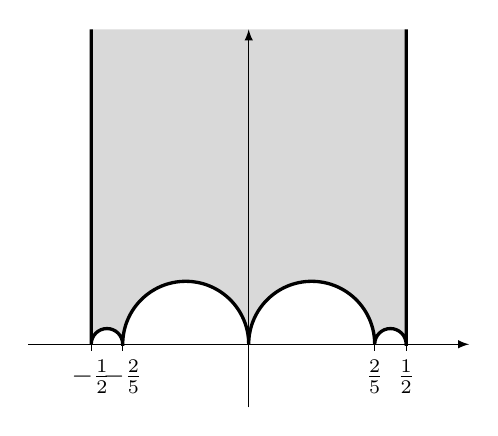
\begin{tikzpicture}[scale=4]
    \draw[very thick, fill=gray!30]
        (-.5,1) -- (-.5,0) --
        (-1/2, 0) arc (180:0:1/20) --
        (-2/5, 0) arc (180:0:1/5) --
        (0, 0) arc (180:0:1/5) --
        (2/5, 0) arc (180:0:1/20) --
        (.5, 0) -- (.5,1);
    \draw[-latex] (-0.7,0) -- (0.7,0);
    \draw[-latex] (0,-.2) -- (0,1);
    \draw(-.5,.02)--(-.5,-.02)node[below]{$-\frac{1}{2}$};
    \draw(.5,.02)--(.5,-.02)node[below]{$\frac{1}{2}$};
    \draw(-2/5,.02)--(-2/5,-.02)node[below]{$-\frac{2}{5}$};
    \draw(2/5,.02)--(2/5,-.02)node[below]{$\frac{2}{5}$};
\end{tikzpicture}
\end{center}
They are regular and have widths $5, 5, 1, 1$ respectively.
Consider the following function,
$$
y(\tau) = q \prod_{n = 1}^{\infty} (1 - q^n)^{5 \left(\frac{n}{5}\right)}
$$
where $\left(\frac{n}{5} \right)$ it the Legendre symbol.
The function $y(\tau)$ is a hauptmodul for the group $\Gamma_1(5)$.
Moreover, $y(0) = - \frac{11}{2} + \frac{5}{2} \sqrt{5}, y(\frac{2}{5}) = i\infty, y(\frac{1}{2}) = -\frac{11}{2} - \frac{5}{2} \sqrt{5}, y(i\infty) = 0$.
The function $y(-1/5\tau)$ is again modular with respect to $\Gamma_1(5)$ and one easily checks that
$$
y\left(-\frac{1}{5 \tau}\right) = \frac{\lambda_1 - y(\tau)}{1 + \lambda_1 y(\tau)}, \quad \lambda_1 = -\frac{11}{2} + \frac{5}{2} \sqrt{5}.
$$
So the function
$$
    t(\tau) = y(\tau) \frac{\lambda_1 - y(\tau)}{1 + \lambda_1 y(\tau)}
$$
is invariant under the involution $t \mapsto -1 / 5\tau$.
In a similar way as in Proposition \ref{prop:2.1} one shows,

\begin{proposition}
\label{prop:3.1}
The function $t(\tau)$ maps the shaded open area in the picture below univalently onto the upper half plane and satisfies
$$
    t(i\infty) = 0, \quad t\left(\frac{i}{\sqrt{5}}\right) = (\lambda_2 + \sqrt{1 + \lambda_2^2})^2, \quad t \left(\frac{4}{9} + \frac{i}{9\sqrt{5}}\right) = (\lambda_2 - \sqrt{1 + \lambda_2^2})^2, \quad t\left(\frac{1}{2}\right) = \infty
$$
where $\lambda_2 = \frac{11}{2} - \frac{5}{2} \sqrt{5}$.
\end{proposition}

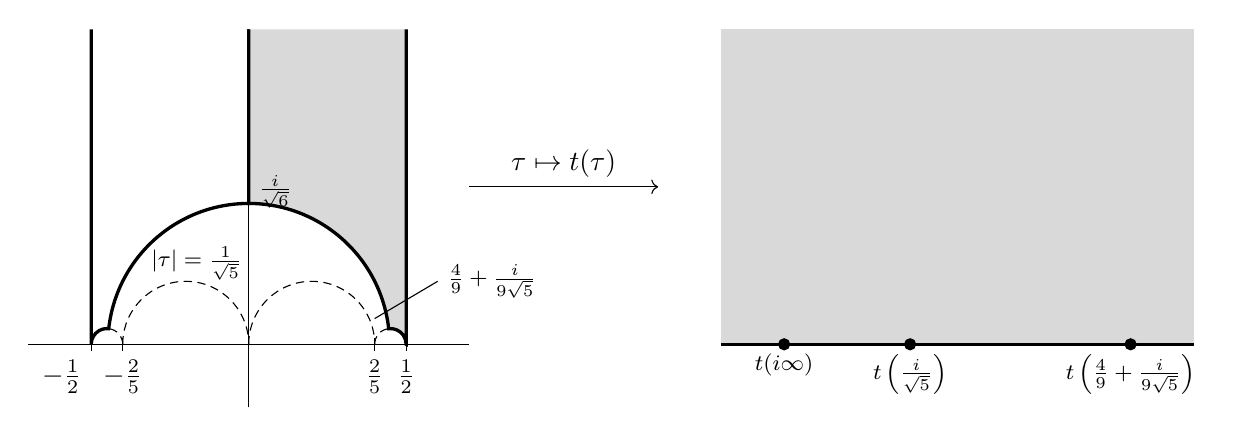
\begin{tikzpicture}[scale=4]
    \draw[very thick]
        (-.5,1) -- (-.5,0) --
        (-1/2, 0) arc (180:78.5:1/20) --
        (-4/9, {1/(9 * sqrt(5))}) arc (173.62:90:{1/sqrt(5)}) --
        (0,{1/sqrt(5)}) -- (0,1);
    \draw[very thick, fill=gray!30]
        (0,1) --
        (0, {1/sqrt(5)}) arc (90:6.38:{1/sqrt(5)}) --
        (4/9, {1/(9 * sqrt(5))}) arc (96.38:0:1/20) --
        (1/2,0) -- (1/2,1);
    \draw (-0.7,0) -- (0.7,0);
    \draw (0,-.2) -- (0,1);
    \draw (0,0.4)node[above right, font=\footnotesize]{$\frac{i}{\sqrt{6}}$};
    \draw[densely dashed] (-2/5, 0) arc (0:83.62:1/20);
    \draw[densely dashed] (-2/5,0) arc (180:0:1/5);
    \draw[densely dashed] (2/5,0) arc (180:96.38:1/20);
    \draw[densely dashed] (0,0) arc (180:0:1/5);
    \draw(-.5,.02)--(-.5,-.02)node[below left]{$-\frac{1}{2}$};
    \draw(.5,.02)--(.5,-.02)node[below]{$\frac{1}{2}$};
    \draw(-2/5,.02)--(-2/5,-.02)node[below]{$-\frac{2}{5}$};
    \draw(2/5,.02)--(2/5,-.02)node[below]{$\frac{2}{5}$};
    \draw (2/5, {1/(5 * sqrt(6))}) -- (0.6,0.2)node[right, font=\footnotesize]{$\frac{4}{9} + \frac{i}{9\sqrt{5}}$};
    % \draw (-0.25, 0.5)node[above]{II};
    % \draw (0.25, 0.5)node[above]{I};
    \draw (-0.34, 0.34)node[below right, font=\footnotesize]{$|\tau| = \frac{1}{\sqrt{5}}$};

    \draw[->] (0.7,0.5) -- (1.3,0.5);
    \draw (1.0, 0.5)node[above]{$\tau \mapsto t(\tau)$};

    \fill[gray!30] (1.5,1.0) -- (1.5,0) -- (3.0, 0) -- (3.0, 1.0);
    \draw[very thick] (1.5,0) -- (3,0);
    \draw[fill] (1.7,0) circle (0.5pt)node[below, font=\footnotesize]{$t(i\infty)$};
    \draw[fill] (2.1,0) circle (0.5pt)node[below, font=\footnotesize]{$t\left(\frac{i}{\sqrt{5}}\right)$};
    \draw[fill] (2.8,0) circle (0.5pt)node[below, font=\footnotesize]{$t\left(\frac{4}{9}+\frac{i}{9\sqrt{5}}\right)$};
\end{tikzpicture}

We also consider the function
$$
    s(\tau) = y(\tau) \frac{\lambda_2 - y(\tau)}{1 + \lambda_2 y(\tau)}, \quad \lambda_2 = \frac{11}{2} - \frac{5}{2} \sqrt{5}.
$$

\begin{lemma}
    \label{lem:3.2}
    The branching values of $s(\tau)$, as defined in Section 1, read $0, \infty$ and $(\lambda_1 + \sqrt{1 + \lambda_1^2})^2$ where $\lambda_1 = -\frac{11}{2} + \frac{5}{2} \sqrt{5}$.
\end{lemma}

\begin{proof}
    The branching values of $s(\tau)$ are the values of $s(\tau)$ at the cusps or the values at the points $\tau$, $\Im \tau > 0$ where $s'(\tau) = 0$.
    The values at the cusps are $0, \infty$.
    Notice that
    $$
        \frac{s'}{s} = \left(1 + \frac{y}{y - \lambda_2} - \frac{y}{y - \lambda_1}\right) \frac{y'}{y} = \frac{y^2 + (11 - 5\sqrt{5})y - 1}{y^2 + 11 y - 1} \frac{y'}{y}.
    $$
    The function $\frac{y'}{y}$ can only be zero at the cusps $0, \frac{1}{2}$.
    If $y^2 + (11 - 5\sqrt{5})y - 1 = 0$ then $y = \lambda_1 \pm \sqrt{1 + \lambda_1^2}$ which implies $s = (\lambda_1 \pm \sqrt{1 + \lambda_1^2})^2$.
\end{proof}

Notice that the $q$-expansions of $t(\tau)$, $s(\tau)$ read
$$
    t(\tau) = \sum_{n=1}^{\infty} a_n q^n, \quad s(\tau) = \sum_{n=1}^{\infty} b_n q^n
$$
where $a_n, b_n$ are algebraic integers in $\bQ(\sqrt{5})$.
From the construction follows that for every $n$ the numbers $a_n, b_n$ are conjugates.

\begin{theorem}
    \label{thm:4}
    Let $L(3, \chi) = \sum_{n=1}^{\infty} \left(\frac{n}{5}\right) n^{-3}$, where $\left(\frac{n}{5}\right)$ is the Legendre symbol.
    Then $8\zeta(3) - 5\sqrt{5}L(3, \chi)$ is not in $\bQ(\sqrt{5})$.
\end{theorem}

\begin{proof}
    Consider the weight 4 form on $\Gamma_1(5)$ given by
    $$
        24 F(\tau) = E_4(\tau) - 25 E_4(5\tau) + 24(E_4(\chi, \tau) - 5\sqrt{5} F_4(\chi, \tau))
    $$
    where
    \begin{align*}
        E_4(\chi, \tau) &= 1 + \sum_{n=1}^{\infty} \left(\frac{n}{5}\right) \frac{n^3 q^n}{1 - q^n}, \\
        F_4(\chi, \tau) &= \sum_{m, n=1}^{\infty} \left(\frac{n}{5}\right) m^3  q^{mn}.
    \end{align*}
    Note that up to a constant factor, $F(\tau)$ is cahracterised by the facts $F(\tau) \in \rM_4(\Gamma_1(5))$, $F(i\infty) = 0$, $F(-\frac{1}{5\tau}) = -25 \tau^4 F(\tau)$.
    The corresponding Dirichlet series reads
    $$
        L(F, s) = 10 (1 - 5^{2-s})\zeta(s) \zeta(s - 3) + \zeta(s) L(s - 3, \chi) - 5\sqrt{5} \zeta(s - 3) L(s, \chi)
    $$
    where
    $$
        L(s, \chi) = \sum_{n=1}^{\infty} \left(\frac{n}{5}\right) n^{-s}.
    $$
    Define $f(\tau)$ by $f(i\infty) = 0$, $(\frac{\dd}{\dd \tau})^{3} f(\tau) = (2\pi i)^3 F(\tau)$.
    then, from Proposition \ref{prop:1.2} follows that
    $$
        5 \tau^2 \left(f\left(-\frac{1}{5\tau}\right) - A\right) = - (f(\tau) - A)
    $$
    where
    \begin{align*}
        A &= 10\left(1 - \frac{1}{5}\right) \zeta(3) \zeta(0) + \zeta(3) L(0, \chi) - 5\sqrt{5} \zeta(0) L(3, \chi) \\
        &= -\frac{1}{3} (8\zeta(3) - 5\sqrt{5} L(3, \chi)).
    \end{align*}
    Now let 
    $$
        -8 E(\tau) = E_2(\tau) - 5 E_2(5\tau) + 20 (E_2(\chi, \tau) - \sqrt{5} F_2(\chi, \tau))
    $$
    where
    \begin{align*}
        E_2(\chi, \tau) &= -\frac{1}{5} + \sum_{n=1}^{\infty} \left(\frac{n}{5}\right) \frac{n q^n}{1 - q^n}, \\
        F_2(\chi, \tau) &= \sum_{m, n=1}^{\infty} \left(\frac{n}{5}\right) m q^{mn}.
    \end{align*}
    The function $E(\tau)$ satisfies $E(-\frac{1}{5\tau}) = -5\tau^2 E(\tau)$, hence $E(\tau) (f(\tau) - A)$ is fixed under the involution $\tau \mapsto -1/5\tau$.
    Consider $E(\tau)$ and $E(\tau)f(\tau)$ as functions of $t = t(\tau)$ and write
    $$
        E(\tau)f(\tau) = \sum_{n=1}^{\infty} c_n q^n, \quad E(\tau) = \sum_{n=1}^{\infty} d_n q^n.
    $$
    By construction it follows that $d_n$ and $[1, \dots, n]^3 c_n$ are algebraic integers in $\bQ(\sqrt{5})$.
    Just as in the proof of Theorem \ref{thm:1}, we observe that the radius of convergence of $E(t)(f(t) - A)$ equals $(\lambda_2 + \sqrt{1 + \lambda_2^2})^2$\footnote{There's a typo in the original article: sign is fixed.} and hence for all $\epsilon > 0$,
    \begin{equation}
        \label{eqn:5}
        |c_n - A d_n| < (\lambda_2 + \sqrt{1 + \lambda_2^2})^{(2 - \epsilon)n} \quad \forall n > n_0(\epsilon).
    \end{equation}
    Now consider the functions
    $$
        24 \overline{F}(\tau) = E_4(\tau) - 25 E_4(5\tau) + 24(E_4(\chi, \tau) + 5\sqrt{5} F_4(\chi, \tau)) 
    $$
    the corresponding third primitive $\overline{f}(\tau)$ and
    $$
        -8 \overline{E}(\tau) = E_2(\tau) - 5 E_2(5\tau) + 20 (E_2(\chi, \tau) + \sqrt{5} F_2(\chi, \tau)).
    $$
    Consider them as functions of $s = s(\tau)$ and write
    $$
        \overline{E}(\tau) \overline{f}(\tau) = \sum_{n=1}^{\infty} \overline{c}_n q^n, \quad \overline{E}(\tau) = \sum_{n=1}^{\infty} \overline{d}_n q^n.
    $$
    From the construction follows that $\overline{c}_n, \overline{d}_n$ are conjugates of $c_n, d_n$ respectively.
    By Lemma \ref{lem:3.2} the smallest nonzero branching value of $s(\tau)$ equals $(-\lambda_1 + \sqrt{1 + \lambda_1^2})^{2}$ and hence the radius of convergence of both $\sum_{n=1}^{\infty} \overline{c}_{n} s^n$ and $\sum_{n=1}^{\infty} \overline{d}_{n} s^n$ is at least $(-\lambda_1 + \sqrt{1 + \lambda_1^2})^{2}$.
    Hence for any $\theta \in \bC$ and any $\epsilon > 0$
    \begin{equation}
        \label{eqn:6}
        |\overline{c}_n - \theta \overline{d}_n| < (\lambda_1 + \sqrt{1 + \lambda_1^2})^{(2 + \epsilon) n} \quad \forall n > n_1(\epsilon, \theta).
    \end{equation}
    Now suppose $A \not\in \bQ(\sqrt{5})$.
    Let $\overline{A}$ be its conjugate and let $d$ be its denominator.
    Multiplication of \eqref{eqn:5} and \eqref{eqn:6} with $\theta = \overline{A}$ yields
    \begin{equation}
        \label{eqn:7}
        |c_n \overline{c}_n - (c_n \overline{d}_n \overline{A} + \overline{c}_n d_n A) + d_n \overline{d}_n A\overline{A}| < \left(\frac{1}{20.3}\right)^{2n} \quad \forall n > n_0.
    \end{equation}
    Since $c_n \overline{c}_n \in \bZ / [1, \dots, n]^{6}$, $c_n \overline{D}_n \overline{A} + \overline{c}_n d_n A \in \bZ / d[1, \dots, n]^{3}$, $d_n \overline{d}_n A \overline{A} \in \bZ / d^2$ and $d^2 [1, \dots, n]^6 < (20.1)^{2n} < (20.3)^{2n}$ for sufficiently large $n$.
    Hence $c_n - d_n A = 0$ for $n$ large enough, and we have a contradiction.
    Theorem \ref{thm:4} now follows.
\end{proof}

\begin{remark*}
By some tedius calculation one can veritfy that the numbers $d_n$ satisfy the recurrence relation 
\begin{align*}
    (n + 1)^{3} d_{n+1} &= ((124 + 55\sqrt{5})n(n+1) + 34 + 15\sqrt{5}) (2n + 1)d_n - n^3 d_{n-1} \\
    d_0 = 1, d_1 &= 34 + 15\sqrt{5}, d_2 = 7111 + 3180 \sqrt{5}, d_3 = 2040334 + 912465\sqrt{5}.
\end{align*}
\end{remark*}

\begin{theorem}
    \label{thm:5}
    The number $\zeta(2) = \frac{\pi^2}{6}$ is irrational.
    \end{theorem}
\begin{proof}
    Consider the function
    $$
        \frac{2i}{5} F(\tau) = (2 + i) E_3(\chi, \tau) - (2 - i) E_3(\chi, \tau)
    $$
    where
    $$
        E_3(\chi, \tau) = \frac{-2 + i}{5} + \sum_{i=1}^{\infty} \chi(k) \frac{k^2 q^k}{1 - q^k}
    $$
    and $\chi(k)$ is the odd character modulo 5 given by $\chi(2) = -i$ and $\overline{\chi}$ is its complex conjugate.
    Then $F(\tau) \in \rM_3(\Gamma_1(5))$, and, in particular, $F(\frac{\tau}{5\tau + 1}) = (5\tau + 1)^{3} F(\tau)$.
    Let $f(\tau)$ be the Fourier series determined by $f(i\infty) = 0$ and $(\frac{\dd}{\dd \tau})^{2} f(\tau) = (2 \pi i)^{2} F(\tau)$.
    In a straightforward manner one can verify that
    $$
        (5\tau + 1)\left(f\left(\frac{\tau}{5\tau + 1}\right) - L(F, 2)\right)= f(\tau) - L(F, 2)
    $$
    where
    $$
        L(F, 2) = \frac{5}{2i} \zeta(2) ((2 + i)L(0, \chi) - (2 - i) L(0, \overline{\chi})) = \zeta(2).
    $$
    Consider also
    $$
        E(\tau) = \frac{3 + i}{2} E_1(\chi, \tau) + \frac{3 - i}{2} E_1(\overline{\chi}, \tau)
    $$
    where
    $$
        E_1(\chi, \tau) = \frac{3 - i}{10} + \sum_{k=1}^{\infty} \chi(k) \frac{q^k}{1 - q^k}.
    $$
    Then $E(\tau) \in \rM_1(\Gamma_1(5))$ and we obtain
    $$
        E\left(\frac{\tau}{5\tau + 1}\right) \left(f\left(\frac{\tau}{5\tau + 1}\right) - \zeta(2)\right) = E(\tau) (f(\tau) - \zeta(2)).
    $$
    This implies that $E(\tau)(f(\tau) - \zeta(2))$ considered as function of $y(\tau)$ does not branch above $y = -\frac{11}{2} + \frac{5}{2}\sqrt{5}$, corresponding to $\tau = 0$.
    Hence $E(\tau)(f(\tau) - \zeta(2))$ as a function of $y$ is a Taylor series in $y$ with radius of convergence $\frac{11}{2} + \frac{5}{2}\sqrt{5}$.
    Note that by construction $E(\tau)$ has a $y$-expansion with integral coefficients, and the $n$th coefficient in the $y$-expansion of $E(\tau)f(\tau)$ is rational with a denominator that divides $[1, \dots, n]^{2}$.
    Out standard argument now yields $\zeta(2) \not\in \bQ$.
\end{proof}

\begin{remark*}
Notice that $E(t) = 1 + 3t + 19 t^2 + 147 t^3 + \cdots$ and the numbers $1, 3, 19, 147, \dots$ correspond exactly to Ap\'ery's numbers for $\zeta(2)$.
The function $E(\tau)$ is also discussed in \cite[p59]{beukers1985some}.
\end{remark*}





% --- Bibliography ---

% Start a bibliography with one item.
% Citation example: "\cite{williams}".

\bibliographystyle{acm} % We choose the "plain" reference style
\bibliography{refs} % Entries are in the refs.bib file


% \begin{thebibliography}{1}

% \bibitem{williams}
%    Williams, David.
%    \textit{Probability with Martingales}.
%    Cambridge University Press, 1991.
%    Print.

% % Uncomment the following lines to include a webpage
% % \bibitem{webpage1}
% %   LastName, FirstName. ``Webpage Title''.
% %   WebsiteName, OrganizationName.
% %   Online; accessed Month Date, Year.\\
% %   \texttt{www.URLhere.com}

% \end{thebibliography}

% --- Document ends here ---

\end{document}